\documentclass[UTF8,zihao=-4]{ctexart}
\usepackage[a4paper,top=1.9cm,bottom=1.8cm,left=2.0cm,right=2.0cm]{geometry}
\usepackage{amsmath,amssymb,booktabs,array,xcolor,fancyhdr,graphicx,tikz}
\usetikzlibrary{arrows.meta,positioning}
\usepackage[hidelinks]{hyperref}
\setCJKmainfont[BoldFont=SimHei]{SimSun}
\setmainfont{Times New Roman}
\definecolor{inkblue}{HTML}{17456D}
\definecolor{redaccent}{HTML}{B51C3B}
\definecolor{softgray}{HTML}{58616A}
\definecolor{paleblue}{HTML}{EEF4F8}
\setlength{\parindent}{0pt}
\setlength{\parskip}{0.35em}
\renewcommand{\baselinestretch}{1.12}
\ctexset{section={format=\large\bfseries\color{inkblue},beforeskip=0.7em,afterskip=0.4em},subsection={format=\normalsize\bfseries,beforeskip=0.6em,afterskip=0.3em}}
\pagestyle{fancy}\fancyhf{}
\fancyhead[L]{\small\color{softgray}毕业论文选题交流}
\fancyhead[R]{\small\color{softgray}策略模型与初步回测}
\fancyfoot[C]{\small\thepage}
\setlength{\headheight}{15pt}
\graphicspath{{../../results/figures/}}
\newcommand{\note}[1]{{\small\color{softgray}#1\par}}
\newcommand{\askbox}[1]{\par\smallskip\colorbox{paleblue}{\parbox{\dimexpr\linewidth-2\fboxsep\relax}{\small #1}}\par}
\begin{document}
\begin{center}
{\fontsize{18}{23}\selectfont\bfseries\color{inkblue}基于宽松风险平价的多资产 ETF 配置研究}\\[0.35em]
{\normalsize 实习中整理的策略思路与当前实现}
\end{center}
\askbox{\textbf{目前进度}\quad 策略代码与初步回测已完成，现就模型设定与实证安排请老师指导。}

\section*{一、策略模型}
\note{思路来源于实习中对桥水风险分散理念的整理。当前实现采用境内上市 ETF，多头、满仓、无杠杆，按周调整配置。以下省略调仓日下标。}
策略希望回答一个具体问题。在风险预算组合的基础上，能否进一步降低波动，同时控制预测收益的损失？为此，先建立风险分散的参考组合，再通过第二步优化调整资金权重。
两步在同一个调仓日依次完成。第一步输出参考权重 $q$，第二步输出实际使用的目标权重 $w$；计算过程中使用同一时点以前的信息。

\subsection*{1. 先求风险预算参考组合}
\textbf{输入与目的。} 输入为当期合格资产的年化协方差矩阵 $\Sigma$ 和风险预算 $b$。$\Sigma$ 同时反映各资产的波动及其共同变化；$b_i$ 表示希望由资产 $i$ 承担的风险份额。当前采用等风险预算 $b_i=1/n$，其中 $n$ 为当期合格资产数。这一步只使用风险信息，不使用收益预测。

\textbf{如何计算。} 在 CVXPY 中定义正的辅助变量 $x$，求解下面的对数风险预算问题，再将求得的 $x^*$ 归一化为资金权重 $q$。
\[
 x^*=\arg\min_{x_i>0}\Bigl\{
 \underbrace{\frac12x^\top\Sigma x}_{\text{控制风险规模}}
 +\underbrace{\left(-\sum_{i=1}^n b_i\log x_i\right)}_{\substack{\text{引入风险预算}\\\text{避免正预算资产的 }x_i\text{ 趋零}}}\Bigr\}.
\]
\[
 \underbrace{q_i=\frac{x_i^*}{\sum_jx_j^*}}_{\text{归一化为资金权重}},\qquad
 \underbrace{b_i=\frac1n}_{\text{等风险预算}},\qquad
 \underbrace{\frac{q_i(\Sigma q)_i}{q^\top\Sigma q}=b_i}_{\text{各资产按预算承担估计风险}}.
\]
\textbf{各项为何这样设置。} 二次项随风险规模增大而增加。负对数项在某个 $x_i$ 趋于零时趋于无穷，使正预算资产保留正的配置；其中的系数 $b_i$ 决定目标风险份额。$x$ 不必加总为 1，归一化后才得到可以持有的资金比例。

在所用协方差正定时，内部最优点满足
\[
 \underbrace{(\Sigma x^*)_i-b_i/x_i^*=0}_{\text{目标函数对 }x_i\text{ 的一阶条件}}
 \quad\Longrightarrow\quad x_i^*(\Sigma x^*)_i=b_i.
\]
归一化保留各资产的风险贡献比例，因此得到上式中的等风险预算关系。这里的风险贡献均基于当期估计的 $\Sigma$，未来实现的风险分配可能不同。


\clearpage
\section*{一、策略模型（续）}
\subsection*{2. 再求最终配置权重}
\textbf{输入与目的。} 固定第一步得到的 $q$，加入预测年化收益率 $\mu$，并令收益目标 $R=\mu^\top q$。第二步希望在尽量保留参考配置的同时降低方差，并控制调整带来的预测收益损失。
\begin{align*}
 \min_w J(w)
 &=\underbrace{\|w-q\|_2^2}_{\substack{\text{尽量保留参考配置}\\\text{衡量资金权重距离}}}
 +\underbrace{\lambda_v\frac{w^\top\Sigma w}{v}}_{\substack{\text{降低组合方差}\\\lambda_v\text{ 控制风险惩罚强度}}}\\[0.3em]
 &\quad+\underbrace{\lambda_r\left[\max\left(0,\frac{R-\mu^\top w}{s}\right)\right]^2}_{\substack{\text{惩罚低于目标的预测收益，达标时为零}\\\lambda_r\text{ 控制收益短缺惩罚强度}}}.
\end{align*}
\[
 \underbrace{\mathbf1^\top w=1}_{\text{全部资金投入}},\qquad
 \underbrace{w_i\ge0}_{\text{不卖空，可为零}},\qquad
 \underbrace{R=\mu^\top q}_{\text{以参考组合预测收益为目标}}.
\]
\note{$w$ 为最终资金权重，$\mu$ 为预测年化收益率，$\Sigma$ 为年化协方差，$\mathbf1$ 为全 1 向量。$\lambda_v,\lambda_r\ge0$；跟踪项系数固定为 1。}
\textbf{参考跟踪项。} $\|w-q\|_2^2$ 将最终配置保持在参考组合附近，为调整设置代价。它衡量的是资金权重距离，因此还需单独查看调整后的风险贡献，不能直接把接近 $q$ 等同于严格风险平价。

\textbf{方差与收益短缺。} 方差项倾向于选择估计风险更低的权重。收益短缺项只在 $\mu^\top w<R$ 时产生惩罚，达到目标后便为零。它允许一定收益损失，避免为满足硬收益约束而失去调整空间；也不会继续奖励超出目标的预测收益。
\[
 \underbrace{v=\max(e^\top\Sigma e,\varepsilon_v)}_{\text{用等权方差统一风险量级}},\qquad
 \underbrace{s=\max(|R|,\max_i|\mu_i|,\varepsilon_m)}_{\text{用预测收益量级归一化短缺}}.
\]
\note{$e=\mathbf1/n$；$\varepsilon_v,\varepsilon_m$ 为防止除零的正下限。输入与尺度在当次求解前固定。}
\textbf{尺度与参数。} $v,s$ 用于统一量级，使两项惩罚无量纲。$\lambda_v$ 决定对方差的重视程度，$\lambda_r$ 决定对预测收益短缺的容忍程度。它们由历史区间年度选定，本次优化仅求权重，求解器不会同时自行选择这两个系数。

\textbf{为什么会偏离参考组合。} 当 $w=q$ 时，跟踪项和收益短缺项均为零。方差项提供离开参考点的动因，另外两项则限制偏离及其收益代价。因此，若去掉方差项，最优权重就回到 $q$。

\askbox{\textbf{“宽松”的含义}\quad 允许最终权重偏离参考组合。收益目标采用软惩罚，风险贡献不再要求严格相等；预测收益目标也不代表实际收益保证。}

\clearpage
\section*{二、策略如何运行与求解}
\subsection*{每周的完整流程}
\begin{center}
\begin{tikzpicture}[
 box/.style={draw=inkblue!45,fill=paleblue,rounded corners=3pt,align=center,text width=4.55cm,minimum height=1.2cm,font=\small},
 arr/.style={-{Stealth[length=2mm]},thick,draw=inkblue},node distance=0.5cm and 0.65cm]
 \node[box](a){\textbf{历史数据与合格资产}\\30 只 ETF，按可用性筛选\\只使用调仓日前的信息};
 \node[box,right=of a](b){\textbf{估计收益与协方差}\\指数加权均值 $\mu$\\收缩协方差 $\Sigma$};
 \node[box,right=of b](c){\textbf{风险预算参考}\\求解对数风险预算问题\\归一化得到 $q$};
 \node[box,below=of c](d){\textbf{最终权重优化}\\输入 $q,\mu,\Sigma,\lambda_v,\lambda_r$\\得到 $w$，检查求解结果};
 \node[box,left=of d](e){\textbf{执行与持有}\\周度调仓，期内权重漂移\\按实际权重变动扣费};
 \node[box,left=of e](f){\textbf{记录回测结果}\\净值、回撤、换手与持仓\\进入下一个调仓周期};
 \draw[arr](a)--(b);\draw[arr](b)--(c);\draw[arr](c)--(d);\draw[arr](d)--(e);\draw[arr](e)--(f);
\end{tikzpicture}
\end{center}

{\small\renewcommand{\arraystretch}{1.25}
\begin{tabular}{@{}p{2.4cm}p{13.7cm}@{}}
\toprule
数据输入 & 股票、债券、货币市场、商品及海外权益 ETF；至少 60 个历史有效观察且方差为正，上市前不回填。\\
估计设置 & 最多使用此前 252 个交易日；均值采用 20 日半衰期 EWMA；协方差采用 Ledoit--Wolf 收缩并作正定数值处理。\\
年度参数 & 较早 252 日形成 $3\times3$ 候选网格，随后 252 日按扣费表现筛选；两段均早于生效日，选定后固定一年。\\
交易成本 & 单边 3 bp，按买卖绝对权重变化之和扣减；成本进入回测，当前目标函数未直接惩罚换手。\\
\bottomrule
\end{tabular}}

\subsection*{已经使用 CVXPY 实现}
\[
 \underbrace{\text{CVXPY}}_{\text{表达目标与约束，检查凸性规则}}
 \quad\longrightarrow\quad
 \underbrace{\text{CLARABEL}}_{\text{现成数值求解器}}
 \quad\longrightarrow\quad
 \underbrace{q\,,\ w}_{\text{参考权重与最终权重}}.
\]
\note{第一步含对数项，使用支持指数锥的求解器；第二步的正部平方可等价改写为凸二次规划。现有代码通过 CVXPY 建模并调用 CLARABEL。}
\[
 \min_{w,z}\quad
 \underbrace{\|w-q\|_2^2+\lambda_v\frac{w^\top\Sigma w}{v}+\lambda_r z^2}_{\text{二次目标}},
 \qquad
 \underbrace{z\ge0,\ z\ge\frac{R-\mu^\top w}{s}}_{\text{线性约束表达非负收益短缺}}.
\]
\note{同时保留 $\mathbf1^\top w=1,w\ge0$。$z$ 为辅助变量，$\lambda_r>0$ 时最优 $z$ 等于归一化短缺的正部。该改写说明可调用标准 QP 求解器；当前实现保留 CVXPY 的正部平方表达。}

\askbox{\textbf{已有求解记录}\quad 451 次周度求解均返回 \texttt{optimal}，使用 CLARABEL；最大约束误差约 $1.8\times10^{-13}$。数值求解已跑通，投资效果仍需结合回测评价。}
\note{年度参数并非唯一识别的估计值，现有每年九组候选均进入一倍标准误筛选集合。后续会解释参数选择的作用与局限。}

\subsection*{策略设计中希望进一步讨论的地方}
\textbf{收益目标。} 当前用参考组合自身的预测收益作为目标，使其与当期资产和资金约束相容。方差惩罚推动权重离开参考点，收益短缺惩罚则控制调整的收益代价。想请您看看，这样表达风险与收益的取舍是否合适。

\textbf{参数与比较。} 年度更新让惩罚系数随历史数据变化，但也增加了策略复杂度。希望结合固定参数和去掉单项目标的对照，判断这些设计是否值得保留；与简单配置比较时，也需解释风险暴露差异。

\clearpage
\section*{三、已经得到的初步回测结果}
\note{评价区间 2018-01-02 至 2026-10-23；五种配置均按周调仓，扣单边 3 bp 成本，252 日年化，$r_f=0$。红色实线为本文策略 Global RRP。}
\begin{center}
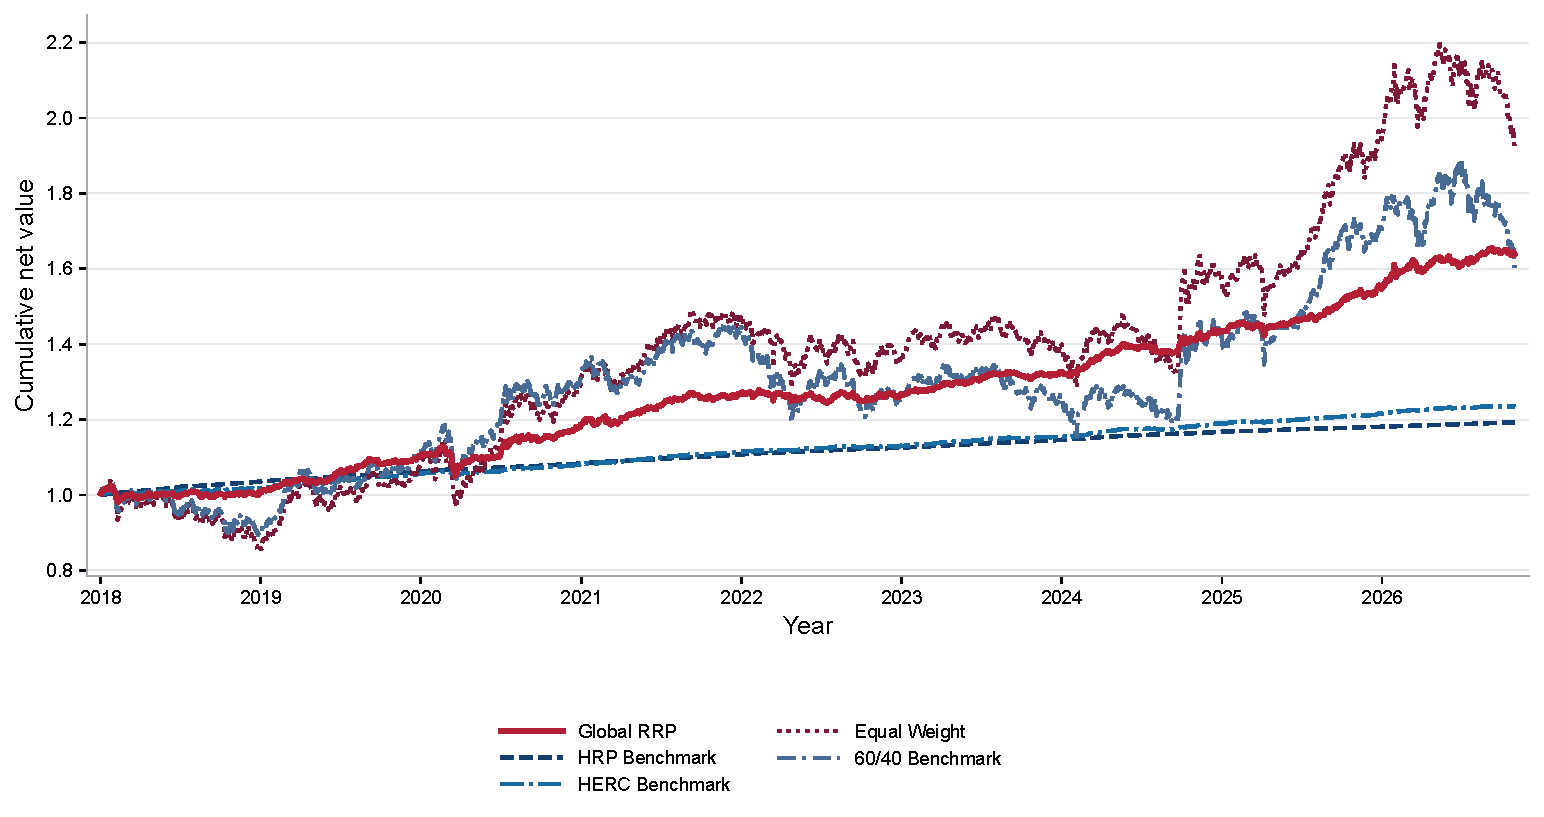
\includegraphics[width=0.87\linewidth]{global_rrp_nav_comparison.pdf}\par
{\small\textbf{图 1}\quad 扣费后的累计净值}\par\vspace{0.2em}
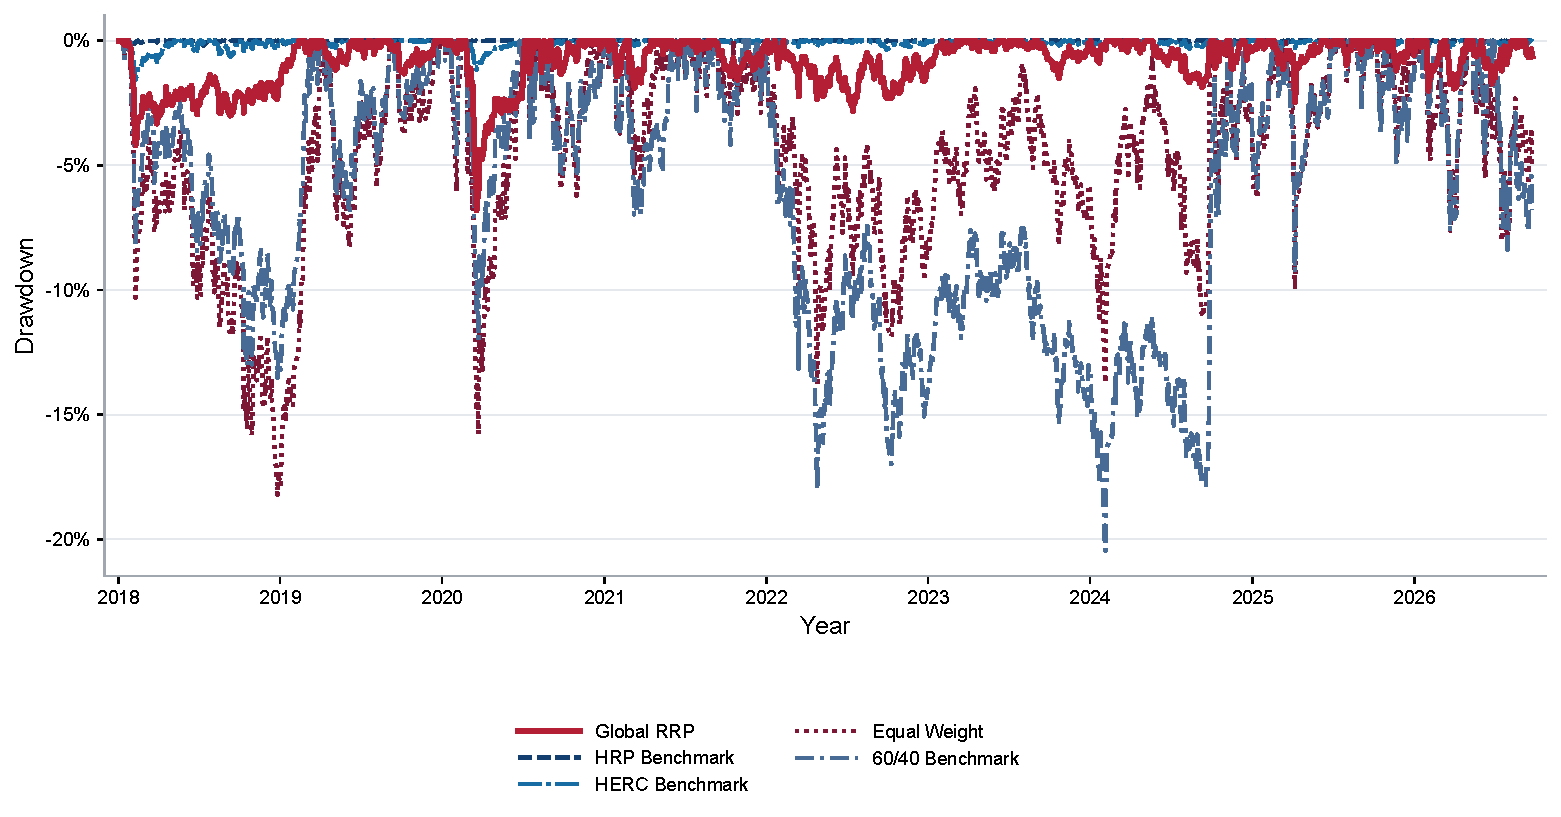
\includegraphics[width=0.87\linewidth]{global_rrp_drawdown_comparison.pdf}\par
{\small\textbf{图 2}\quad 从历史净值高点计算的回撤}\par
\end{center}
\vspace{-0.25em}
{\small\renewcommand{\arraystretch}{1.12}\centering
\begin{tabular}{@{}lrrrr@{}}
\toprule
配置方法 & 净年化收益 & 年化波动 & 夏普比率 & 最大回撤\\
\midrule
\textbf{Global RRP} & \textbf{5.97\%} & \textbf{3.58\%} & \textbf{1.636} & \textbf{$-6.80\%$}\\
HRP Benchmark & 2.09\% & 0.26\% & 7.834 & $-0.19\%$\\
HERC Benchmark & 2.51\% & 0.81\% & 3.073 & $-1.57\%$\\
Equal Weight & 8.29\% & 13.13\% & 0.673 & $-18.23\%$\\
60/40 Benchmark & 6.12\% & 12.07\% & 0.553 & $-20.46\%$\\
\bottomrule
\end{tabular}\par}
\note{当前策略月均换手 17.28\%，平均货币 ETF 权重 18.02\%；货币 ETF 与三只国债、信用债 ETF 合计平均权重 66.36\%。收益与风险差异需结合资产暴露解释，以上为历史回测结果。}
\clearpage
\section*{四、希望请老师指导的问题}
目前已完成这套策略的代码实现与初步回测，想请您看看，是否可以在此基础上开展本科毕业论文研究，以及策略中还有哪些需要调整的地方。

\textbf{模型设定。} 以风险预算组合为参考，加入方差和预测收益短缺惩罚，这样的研究思路是否合适？收益目标或惩罚形式是否需要修改？

\textbf{参数选择。} 当前采用年度更新的惩罚系数，是否有必要简化为固定参数，或采用其他选择方式？

\textbf{实证安排。} 现有对照方法是否足以评价策略效果，还需要优先补充哪些比较或检验？
\end{document}
